\newpage
\section{Интегральная формула Коши для функции и ее производных.}


\textbf{Интегральная формула Коши для голоморфных функций:}

Пусть $D$ --- односвязная область в $\mathbb{C}$, $\partial D$ --- граница $D$, $f\in H(D\cup \partial D).$

Тогда для $z_0 \in D$:
$$f(z_0)=\frac{1}{2\pi i} \cdot \oint\limits_{\partial D} \frac{f(z)}{z-z_0}dz$$

\begin{proof}
    \ \\
    \begin{figure}[!ht]
        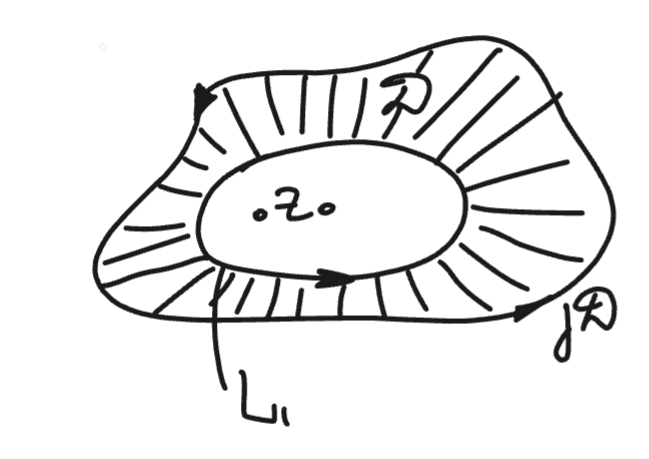
\includegraphics[scale=0.6]{answers/img/ans9.png}
    \end{figure}\\
    1) Пусть $L_1$ -- простой контур, $L_1 \subset D$\\
    Пусть $D_1$ -- область внутри $L_1$, $G=D\backslash D_1\backslash L_1$ -- многосвязная область\\
    По т. Коши для многосвязной области:
    $$\int\limits_{\partial G}\frac{f(z)}{z-z_0}dz=0,$$
    т.к. $\frac{f(z)}{z-z_0} \in H(G)$\\
    Имеем $\partial G = \partial D \cup (-L_1)$:\\
    $$\oint\limits_{\partial D}\frac{f(z)}{z-z_0}dz-\oint\limits_{L}\frac{f(z)}{z-z_0}dz=0$$

    2) Пусть $\gamma: \, z=z+r\cdot e^{it}, \ t\in[0, 2\pi], \ r>0$\\
    $f(z)=(z-a)^n; \ n\in \mathbb{Z}$\\
    $\int\limits_{\gamma}(z-a)^n dz = \int\limits_0^{2\pi} (a+r\cdot e^{it}-a)^n\cdot r\cdot ie^{it}dt = r^{n+1}\cdot i \cdot \int\limits_0^{2\pi} e^{it(n+1)}dt \Rightarrow$\\
    $\Rightarrow \oint\limits_{L_1}\frac{dz}{z-z_0} = 2\pi i,$
    где $L_1$ -- окр-ть с центром в точке $z_0$\\

    3) Пусть $\sigma_1$ -- радиус $L_1$ и $L_1 \subset D$\\
    $I = \left| \frac{1}{2\pi i } \oint\limits_{L_1} \frac{f(z)}{z-z_0}dz-f(z_0) \right| = \left| \frac{1}{2\pi i} \oint\limits_{L_1} \frac{f)(z)}{z-z_0}dz - f(z_0)\frac{1}{2\pi i}\int\limits_{L_1} \frac{dz}{z-z_0}\right| = $\\
    $= \left| \frac{1}{2\pi i}\oint\limits_{L_1} \frac{f(z)-f(z_0)}{z-z_0}dz \right| \leq \frac{1}{2\pi |i|} \oint\limits_{L_1}\left| \frac{f(z)-f(z_0)}{z-z_0} \right||z'(t)|dt$\\

    4) Так как $f \in H(D)$, то $\forall \varepsilon > 0 \, \exists \delta (\varepsilon)>0: \, |z-z_0|<\delta \rightarrow |f(z)-f(z_0)|<\varepsilon$\\
    Имеем $z\in L_1: \ |z-z_0| = \sigma_1$:\\
    $\left| \frac{f(z)-f(z_0)}{z-z_0} \right|< \frac{\varepsilon}{\sigma_1}: \ \oint\limits_{L_1}|z'(t)|dt$ -- длина $L_1$, то есть $2\pi \sigma_1$\\
    Тогда $I \leq \frac{1}{2\pi}\cdot \frac{\varepsilon}{\gamma_1}\cdot 2\pi \sigma_1 = \varepsilon \Rightarrow$ не зависит от $\varepsilon$ 

\end{proof}
\textbf{Интегральная формула Коши для производных:}

Пусть $f\in H(D): \ G\cup \partial G \subset D; \ D$ --- область, ограниченная конечным числом замкнутых кривых, $z_0 \in G$

Тогда:
$$f^{(n)}(z_0) = \frac{n!}{2\pi i} \int\limits_{\partial G}\frac{f(\xi)}{(\xi-z_0)^{n+1}}d\xi$$

\begin{proof}
    \ \\
    По теоремам о разложении голоморфной функции в степенной ряд и теореме о единственности разложения в степенной ряд:\\
    $c_n=\frac{1}{2\pi} \oint\limits_{{\gamma}_r} \frac{f(\xi)d\xi}{(\xi-z_0)^{n+1}}$ \\[2mm]
    $f^{(n)}(z_0) = c_n n! = \frac{n!}{2 \pi i}\int \limits_{{\gamma}_r} \frac{f(\xi)}{(\xi - z_0)^{n+1}}\xi$ \\[2mm]
    $\oint\limits_{{\gamma}_r}\dots=\oint\limits_{\partial G}\dots \Rightarrow$ утверждение теоремы
\end{proof}
